\begin{frame}{Quantum Teleportation}

\bigskip

The IBM quantum computers currently do not support instructions after measurements, meaning we cannot run the quantum teleportation in its current form on real hardware. 

\bigskip

\begin{definition}[Principle of deferred measurement]
Measurements can always be moved from an intermediate stage of a quantum circuit to the end of the circuit.

If the measurement results are used at any stage of the circuit then the \alert{classically controlled operations} can be replaced by \alert{conditional quantum operations}.
\end{definition}

\end{frame}

\begin{frame}{Deferred Measurement}
 
 A consequence of the principle of deferred measurement is that \alert{measurement commutes with control}.
 
 \bigskip
 
\begin{center}
    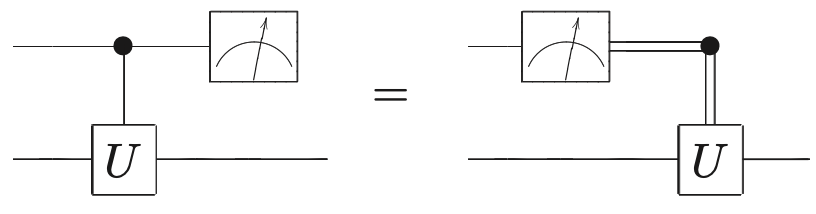
\includegraphics[width=0.85\textwidth]{img/DeferredMeasure.png}
\end{center}

\bigskip

\textbf{Exercise}

Prove the equality of the two circuits depicted above.


\end{frame}

\begin{frame}{Equivalent Teleportation Circuits}
 
\begin{center}
    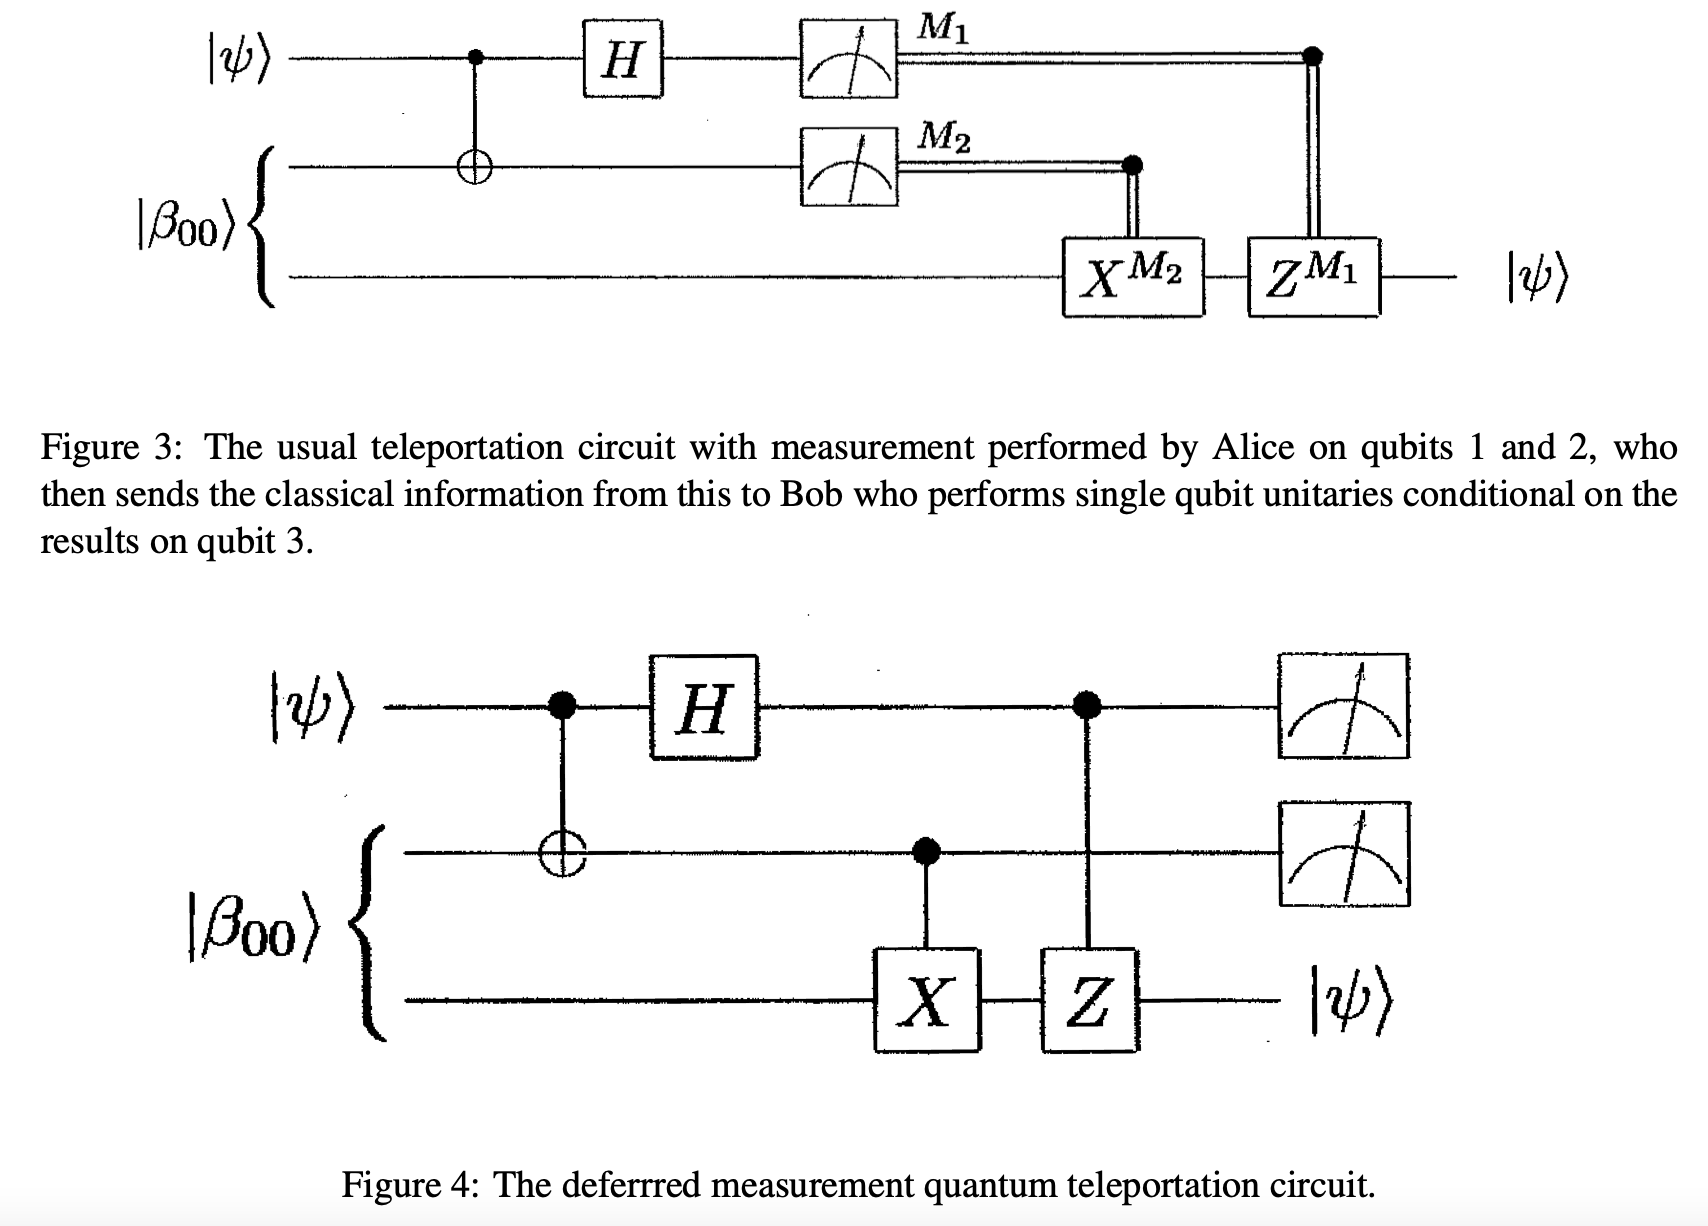
\includegraphics[width=0.80\textwidth]{img/EqivTelCircuits.png}
\end{center}
\end{frame}

\begin{frame}{Teleportation as State Transfer}
We are only interested in taking the input qubit $\psi$ to another location. We do not care what state we get in place of the original qubit at the sender. 

\begin{center}
    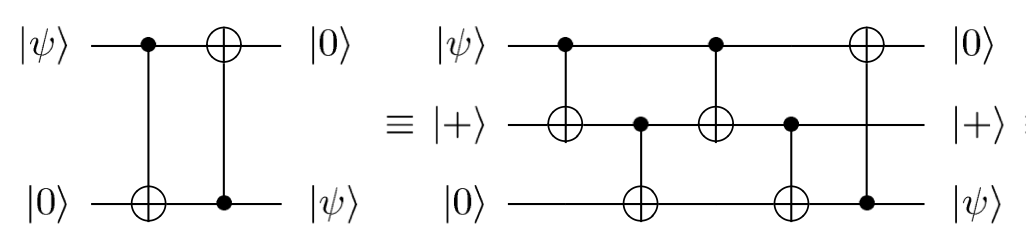
\includegraphics[width=0.80\textwidth]{img/state-transfer.png}
\end{center}

Other equivalent circuits:
\begin{center}
    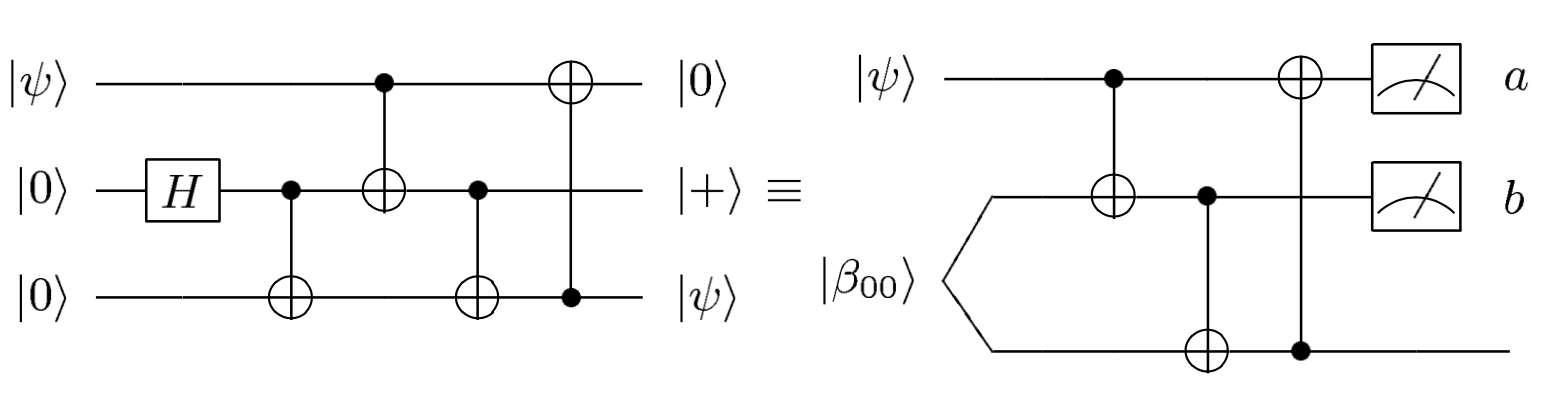
\includegraphics[width=0.80\textwidth]{img/Other-teleportation.png}
\end{center}
\end{frame}